\documentclass[11pt]{article}

\usepackage[final]{acl}
\usepackage{times}
\usepackage{latexsym}
\usepackage[T1]{fontenc}
\usepackage[utf8]{inputenc}
\usepackage{microtype}
\usepackage{booktabs}
\usepackage{amsmath}
\usepackage{graphicx}
\usepackage{inconsolata}

% generated by scripts/make_tables.py -- do not edit
\newcommand{\RGazetteerP}{0.303}
\newcommand{\RGazetteerR}{0.067}
\newcommand{\RGazetteerF}{0.110}
\newcommand{\RGazetteerPF}{0.214}
\newcommand{\RGazetteerType}{0.294}
\newcommand{\RGazetteerHalluc}{0.000}
\newcommand{\RGazetteerAurc}{0.299}
\newcommand{\RGazetteerEce}{0.399}
\newcommand{\RGazetteerCovNinety}{0.011}
\newcommand{\RGazetteerSeconds}{21}
\newcommand{\RChunkerP}{0.178}
\newcommand{\RChunkerR}{0.476}
\newcommand{\RChunkerF}{0.259}
\newcommand{\RChunkerPF}{0.445}
\newcommand{\RChunkerType}{0.388}
\newcommand{\RChunkerHalluc}{0.000}
\newcommand{\RChunkerAurc}{0.590}
\newcommand{\RChunkerEce}{0.634}
\newcommand{\RChunkerCovNinety}{0.000}
\newcommand{\RChunkerSeconds}{53}
\newcommand{\RChunkerGatedP}{0.238}
\newcommand{\RChunkerGatedR}{0.200}
\newcommand{\RChunkerGatedF}{0.217}
\newcommand{\RChunkerGatedPF}{0.402}
\newcommand{\RChunkerGatedType}{0.443}
\newcommand{\RChunkerGatedHalluc}{0.000}
\newcommand{\RChunkerGatedAurc}{0.562}
\newcommand{\RChunkerGatedEce}{0.520}
\newcommand{\RChunkerGatedCovNinety}{0.001}
\newcommand{\RChunkerGatedSeconds}{28}
\newcommand{\RCvalueP}{0.011}
\newcommand{\RCvalueR}{0.006}
\newcommand{\RCvalueF}{0.008}
\newcommand{\RCvaluePF}{0.385}
\newcommand{\RCvalueType}{0.406}
\newcommand{\RCvalueHalluc}{0.000}
\newcommand{\RCvalueAurc}{0.496}
\newcommand{\RCvalueEce}{0.413}
\newcommand{\RCvalueCovNinety}{0.002}
\newcommand{\RCvalueSeconds}{39}
\newcommand{\RUnionP}{0.131}
\newcommand{\RUnionR}{0.363}
\newcommand{\RUnionF}{0.193}
\newcommand{\RUnionPF}{0.440}
\newcommand{\RUnionType}{0.404}
\newcommand{\RUnionHalluc}{0.000}
\newcommand{\RUnionAurc}{0.583}
\newcommand{\RUnionEce}{0.647}
\newcommand{\RUnionCovNinety}{0.001}
\newcommand{\RUnionSeconds}{70}
\newcommand{\RFullP}{0.337}
\newcommand{\RFullR}{0.388}
\newcommand{\RFullF}{0.361}
\newcommand{\RFullPF}{0.548}
\newcommand{\RFullType}{0.595}
\newcommand{\RFullHalluc}{0.000}
\newcommand{\RFullAurc}{0.396}
\newcommand{\RFullEce}{0.308}
\newcommand{\RFullCovNinety}{0.013}
\newcommand{\RFullSeconds}{136}
\newcommand{\RNoNegativeP}{0.285}
\newcommand{\RNoNegativeR}{0.368}
\newcommand{\RNoNegativeF}{0.321}
\newcommand{\RNoNegativePF}{0.569}
\newcommand{\RNoNegativeType}{0.602}
\newcommand{\RNoNegativeHalluc}{0.000}
\newcommand{\RNoNegativeAurc}{0.375}
\newcommand{\RNoNegativeEce}{0.309}
\newcommand{\RNoNegativeCovNinety}{0.011}
\newcommand{\RNoNegativeSeconds}{132}
\newcommand{\RNoConsensusP}{0.331}
\newcommand{\RNoConsensusR}{0.406}
\newcommand{\RNoConsensusF}{0.365}
\newcommand{\RNoConsensusPF}{0.551}
\newcommand{\RNoConsensusType}{0.593}
\newcommand{\RNoConsensusHalluc}{0.000}
\newcommand{\RNoConsensusAurc}{0.404}
\newcommand{\RNoConsensusEce}{0.314}
\newcommand{\RNoConsensusCovNinety}{0.012}
\newcommand{\RNoConsensusSeconds}{135}
\newcommand{\RNoVerifierP}{0.192}
\newcommand{\RNoVerifierR}{0.469}
\newcommand{\RNoVerifierF}{0.272}
\newcommand{\RNoVerifierPF}{0.458}
\newcommand{\RNoVerifierType}{0.399}
\newcommand{\RNoVerifierHalluc}{0.000}
\newcommand{\RNoVerifierAurc}{0.548}
\newcommand{\RNoVerifierEce}{0.612}
\newcommand{\RNoVerifierCovNinety}{0.001}
\newcommand{\RNoVerifierSeconds}{67}
\newcommand{\RNoAbstentionP}{0.307}
\newcommand{\RNoAbstentionR}{0.450}
\newcommand{\RNoAbstentionF}{0.365}
\newcommand{\RNoAbstentionPF}{0.542}
\newcommand{\RNoAbstentionType}{0.597}
\newcommand{\RNoAbstentionHalluc}{0.000}
\newcommand{\RNoAbstentionAurc}{0.422}
\newcommand{\RNoAbstentionEce}{0.268}
\newcommand{\RNoAbstentionCovNinety}{0.010}
\newcommand{\RNoAbstentionSeconds}{137}
\newcommand{\RNoStructureP}{0.350}
\newcommand{\RNoStructureR}{0.368}
\newcommand{\RNoStructureF}{0.358}
\newcommand{\RNoStructurePF}{0.559}
\newcommand{\RNoStructureType}{0.583}
\newcommand{\RNoStructureHalluc}{0.000}
\newcommand{\RNoStructureAurc}{0.363}
\newcommand{\RNoStructureEce}{0.260}
\newcommand{\RNoStructureCovNinety}{0.000}
\newcommand{\RNoStructureSeconds}{137}
\newcommand{\NumDocs}{44}
\newcommand{\NumPapers}{24}
\newcommand{\NumPatents}{20}
\newcommand{\NumGold}{895}
\newcommand{\NumGoldTracked}{819}
\newcommand{\NumGoldPaper}{339}
\newcommand{\NumGoldPatent}{556}
\newcommand{\PctArtifact}{55}


\title{Grounded Extraction of Technology Mentions from Papers and Patents}

\author{}

\begin{document}
\maketitle

\begin{abstract}
Tracking how technologies emerge and spread begins with reading individual
documents and naming the technologies in them. We argue that this apparently
routine extraction task has an unusual error profile once its output is
aggregated into trends: a fabricated technology is not averaged away by scale,
because a spurious term whose rate follows corpus growth produces a curve
indistinguishable from a genuine emerging technology, while a missed mention
mostly rescales a series without changing its shape. We therefore build an
extractor around structural constraints rather than around a confidence
threshold. Every emitted mention is a pair of character offsets into its source
document with a cited evidence sentence, so a model that names a technology we
cannot locate has named nothing; candidates are generated by five deliberately
over-eager recallers and filtered by a guard stack, an independent verifier
cascade and a single calibrated abstention threshold. On a \NumGold-mention gold
set spanning \NumPapers{} arXiv abstracts and \NumPatents{} USPTO publications
across nine technology areas, the full system reaches \RFullPF{} partial F$_1$
at a measured hallucination rate of \RFullHalluc. An ablation over six components
finds only one of them unambiguously load-bearing --- the verifier --- while two
others buy strict precision at a measurable cost in overlap recall and in ranking
quality, which we report rather than smooth over. We also report a negative
result: span grounding bounds but does not close indirect prompt injection,
because an adversary can write their phantom technology into their own patent.
\end{abstract}

\section{Introduction}

A lab that wants to track the evolution of technology through the scientific and
patent literature needs, before anything else, to know which technologies each
document is about. The rest of the pipeline --- time series, emergence detection,
successor analysis --- consumes that output and cannot repair it.

The task looks like scientific named-entity recognition, and the obvious move is
to apply the machinery built for that: a span tagger over a scientific ontology
\cite{augenstein2017scienceie,luan2018scierc}, a domain-pretrained encoder
\cite{beltagy2019scibert}, a span-enumeration model \cite{wadden2019dygiepp,
zhong2021pure}, or a prompted generative extractor. Each of these is a
reasonable starting point and none of them is designed for the property that
matters here.

That property is an asymmetry between the two kinds of error. Suppose an
extractor invents a technology --- a plausible name, a plausible type --- at some
low rate. Downstream, trend detection works by comparing a term's frequency
against a baseline, so a constant spurious rate produces a flat line and does no
harm, but a spurious rate that tracks corpus growth produces a rising line that
is indistinguishable from a real emerging technology and that nobody will go
back and check. A missed mention behaves quite differently: it usually rescales
a series without changing its shape. Precision errors are therefore not merely
more costly than recall errors, they are qualitatively different, and they are
the errors that generative extractors make \cite{ji2023hallucination}.

We take the design consequence seriously. Rather than tune an extractor to be
cautious, we make the failure unrepresentable: a mention is defined as a pair of
character offsets into the source document, its surface form is the slice at
those offsets, and it must cite a sentence from the document that contains it.
A model that returns a technology name we cannot locate has returned nothing.
This is the span-level analogue of attribution work in generation
\cite{rashkin2023attribution,min2023factscore}, applied as a hard gate rather
than as a post-hoc score.

Structural grounding costs recall --- it discards a correct identification that
was paraphrased --- so the rest of the system is built to give that recall back
somewhere it can be checked. Five recallers over-generate on purpose, a guard
stack removes what is provably wrong, an independent verifier cascade challenges
what survives, and a single calibrated threshold decides what to withhold for
human review. Contributions:

\begin{enumerate}\itemsep0pt
\item A precision-dominant formulation of technology extraction for evolution
tracking, with selective prediction \cite{elyaniv2010selective,
geifman2017selective} as its evaluation frame rather than F$_1$ at full coverage.
\item A pipeline in which grounding, evidence and provenance are checked
invariants, evaluated by ablation on both genres.
\item A \NumGold-mention gold set over \NumDocs{} papers and patents spanning
nine technology areas, with annotation guidelines and its limitations stated.
\item An adversarial test suite that drives the pipeline with a deliberately
hostile model, including the negative result on prompt injection in
\S\ref{sec:injection}.
\end{enumerate}

\section{What makes this task not standard NER}
\label{sec:task}

\paragraph{The vocabulary is open by construction.} The point of tracking
technology is to see new technology. An extractor whose output is constrained to
an ontology can never report one, which rules out entity linking as the primary
mechanism and makes a knowledge base an anchor rather than a target. In our gold
set, \PctArtifact\% of mentions are specific artefacts, and the ones that matter
most for tracking --- the document's own contribution --- are by definition the
ones least likely to be in any lexicon.

\paragraph{Granularity is the whole problem in disguise.} ``Machine learning'',
``attention mechanism'' and ``FlashAttention'' are all technologies at different
levels. A tracker that mixes them reports that machine learning is the fastest
growing technology of every year since 1995. We therefore type mentions over a
nine-way ontology that separates artefacts, methods and materials (tracked) from
fields, tasks, metrics, datasets and tools (extracted, annotated, but excluded
from the tracked stream), and record a granularity level.

\paragraph{Stance carries most of the signal.} A mention count conflates a
technology being introduced, used and beaten. We tag each mention as
\textsc{proposed}, \textsc{used}, \textsc{compared}, \textsc{background} or ---
for patents --- \textsc{claimed}, because the shift of a technology's role
distribution from proposed to used is the clearest single indicator of adoption.

\paragraph{The two genres fail differently.} Papers are fluent, citation-dense
and name their contribution explicitly. Patents are deliberately abstract, repeat
component names dozens of times, and bury the invention in claim language whose
purpose is breadth rather than clarity. A lexicon tuned on one is close to
useless on the other; \S\ref{sec:results} quantifies this.

\section{Approach}

\subsection{Structure-aware ingestion}

Normalisation repairs ligatures, line-break hyphenation and typographic
characters, and masks citation markers, while maintaining a per-character map
back into the raw text. Invertibility is not a nicety: when a human audits an
extraction, they must be shown the mention as it appears in the original filing.

Both genres are segmented onto one closed set of structural zones --- title,
abstract, method, related work for papers; field, background, summary, detailed
description and individual claims for patents --- so that a single stance
classifier serves both. Patent claims are split individually and each is
classified as independent or dependent by detecting back-references
(\texttt{of claim 1}), which matters because a term in an independent claim is
being monopolised, not merely discussed.

\subsection{Recall: over-generate on purpose}

Five recallers run over each document, in three cost tiers.

\textbf{Noun-phrase lattice.} Dependency chunks \cite{honnibal2020spacy} are
expanded into a small span lattice: every left truncation after leading vague
modifiers, crossed with alternative noun-final right boundaries. Two failures
forced the second direction. Whether the term is ``string similarity'' or
``superficial string similarity'' depends on information the recaller does not
have; and the parser attaches a following word often enough to matter
(``obstacle-aware route planning grounds''), which no left truncation recovers.

\textbf{Abbreviation mining.} Schwartz--Hearst \cite{schwartz2003abbrev} recovers
the defining parenthetical mention, which is both a high-precision candidate and
the best within-document coreference signal available anywhere in the pipeline.

\textbf{Terminology statistics.} C-value/NC-value \cite{frantzi2000cvalue} is the
only recaller sensitive to \emph{nesting}, which is exactly the granularity
problem; we add a termhood penalty in the spirit of \citet{kageura1996termhood}.

\textbf{Knowledge base.} Aho--Corasick matching against the Computer Science
Ontology \cite{salatino2020cso}. Structurally unable to find anything new, it
earns its place as a consensus witness.

\textbf{Language model.} A tier-2 proposer, run only over zones the cheap tiers
left thin, capped at three windows and 9k characters per document.

We initially gated the chunker on a curated technology head-noun lexicon, which
is the natural design and looks like a precision win. It is not: measured against
gold, gating discards 53\% of mentions before any classifier sees them, because
no lexicon anticipates \emph{highback}, \emph{rule-based elision} or the
mechanical-component vocabulary patents are built from. Table~\ref{tab:baselines}
reports both settings.

\subsection{Grounding as a structural constraint}

Every candidate, from any recaller, must be a verbatim slice of the document at
the offsets it reports. For model-proposed spans this is enforced by relocation:
the cited evidence sentence is grounded first, the surface is then searched
inside it, and a bounded ladder --- exact, whitespace-insensitive,
case-insensitive, and optionally a similarity snap --- returns \emph{the
document's} characters or nothing at all. The ladder rung each accepted span
landed on is recorded; the similarity rung is disabled by default because it is
the only one that can silently move a span onto a different entity.

The resulting invariant is asserted directly in the test suite: for every emitted
mention, \texttt{doc.text[start:end] == surface}. The hallucination rate we
report is consequently a check on the implementation rather than a comparison
between systems, and a non-zero value would be a bug report.

\subsection{Typing, stance and verification}

Type is a linear model over interpretable features: head-noun lexicon
membership, orthography (acronyms, CamelCase, version numbers, chemical
formulae), knowledge-base depth, structural zone, and a distributional back-off
that scores the surface against hand-seeded prototype centroids
\cite{reimers2019sbert}. Linearity is deliberate --- the decision must be
explainable in an audit, and with a few hundred annotated mentions a linear model
is also the better estimator. Stance combines a zone prior with a cue lexicon in
a window around the mention.

Verification is a cascade of three checks of increasing cost, each of which may
abstain. A \emph{structural} verifier re-derives grounding and evidence from the
document rather than trusting the record. An \emph{embedding} verifier gives a
distributional second opinion and decides the easy cases in both directions.
Only the residual uncertainty band reaches an \emph{LLM judge}, which is shown
the evidence sentence, the term and the proposed type --- and nothing about how
any of them were produced, because a verifier shown the proposer's reasoning
ratifies it. Where proposer and verifier disagree and the proposer had
independent support, an adjudicator on a stronger model sees a wider context
window and may accept, reject, or abstain; the prompt pushes it towards
abstention, which for a corpus that will be aggregated costs one annotator-minute
instead of a data point nobody revisits.

\subsection{One abstention mechanism}

An earlier version let each guard abstain independently and remove the mention.
This made recall a function of guard ordering and filled the review queue with
items no one had scored. The system now has exactly one abstention mechanism:
guards either reject (a provable violation) or pass, soft signals feed a logistic
confidence model, and a single calibrated threshold decides what is emitted
versus withheld. Overlapping candidates are resolved \emph{after} scoring, by
confidence, since the only evidence available before typing is span length and
recaller count --- which picks the wrong boundary about as often as the right one.

\subsection{Canonicalisation}

Counting surface forms is not counting technologies. Mentions are merged by a
cascade: in-document abbreviation pairs (promoted to corpus-wide aliases),
knowledge-base identity, lemma-key identity, and finally embedding
agglomeration over the NIL residue with a head-noun compatibility constraint
that prevents ``graph neural network'' and ``spiking neural network'' from
collapsing. Clusters that never touch the ontology receive a stable synthetic
identifier, so an emerging technology can be tracked from first naming and
reconciled with an ontology later.

\subsection{Cost discipline}
\label{sec:cost}

Per-candidate verification calls are the obvious design and the wrong one: a
patent yields $10^2$ candidates whose useful payload is a term, a type and one
sentence. Three reductions apply before anything is sent. Verification is
deduplicated on (surface, type, sentence), so a term repeated forty times in a
specification is one question. Only the embedding verifier's uncertainty band
escalates. Survivors are batched roughly twenty per request behind a cached
system prompt. Together these take a patent from around 120 verifier calls to
one or two. A planner reproduces the window-selection logic to price a run before
any request is issued.

\section{Experimental setup}

\paragraph{Data.} \NumPapers{} arXiv abstracts sampled across six categories
(computational linguistics, machine learning, signal processing, materials
science, applied physics, quantitative biology) and \NumPatents{} USPTO
publications sampled from the HUPD frame \cite{suzgun2023hupd} stratified over
five CPC sections, with full text from Google Patents. The patent sample spans
snowboard bindings, HDAC inhibitors, Talbot--Lau interferometry, Ziegler--Natta
catalysis, wheel bearings and narrowband spread-spectrum transmission. This
spread is the point: a pipeline tuned on one vocabulary would visibly fail on the
others.

\paragraph{Gold.} \NumGold{} mentions over \NumDocs{} documents
(\NumGoldPaper{} paper, \NumGoldPatent{} patent), annotated by one author under
written guidelines. The evaluation zone is title and abstract for papers, plus
the first independent claim for patents, capped at 1400 characters --- Markush
structure claims in chemical cases run to thousands of characters of variable
definitions that name no technology. System output is filtered to the same zone,
so a system is neither rewarded nor penalised outside it.

\paragraph{Metrics.} Strict (exact offsets) and partial (overlap) span P/R/F$_1$;
type accuracy on matched spans; the hallucination rate defined above; and the
area under the risk--coverage curve (AURC, lower is better), which rewards a
system whose errors are concentrated in its low-confidence tail
\cite{geifman2017selective}. We treat partial F$_1$ as the primary comparison
figure, following practice in term extraction \cite{rigoutsterryn2020acter,
qasemizadeh2016aclrdtec}, because boundary choice for technology terms is
genuinely ambiguous and the strict/partial gap measures disagreement about
boundaries rather than failure to find the technology.

\paragraph{Configuration.} All numbers below are from the offline configuration
--- deterministic and neural tiers only, no API key --- so they are reproducible
without cost. Baselines are components of this system rather than external tools,
which answers the question a reader actually has (what does the machinery buy
over its own parts) and avoids comparing against systems built for a different
ontology.

\section{Results}
\label{sec:results}

\begin{table}[t]
\centering\small\setlength{\tabcolsep}{3.5pt}
% generated by scripts/make_tables.py -- do not edit
\begin{tabular}{@{}lrrrrrr@{}}
\toprule
 & \multicolumn{3}{c}{Strict} & \multicolumn{1}{c}{Partial} & & \\
\cmidrule(lr){2-4}\cmidrule(lr){5-5}
System & P & R & F$_1$ & F$_1$ & Type & AURC \\
\midrule
CSO gazetteer & 0.303 & 0.068 & 0.112 & 0.217 & 0.294 & 0.299 \\
Chunker (gated) & 0.227 & 0.193 & 0.208 & 0.395 & 0.442 & 0.568 \\
Chunker (open) & 0.174 & 0.474 & 0.255 & 0.442 & 0.386 & 0.595 \\
C-value/NC-value & 0.004 & 0.002 & 0.003 & 0.368 & 0.399 & 0.520 \\
Union, no guards & 0.127 & 0.358 & 0.188 & 0.434 & 0.402 & 0.591 \\
\bottomrule
\end{tabular}

\caption{Single-recaller baselines. Every row is a configuration of the same
code, with the guard stack reduced to grounding.}
\label{tab:baselines}
\end{table}

\begin{table}[t]
\centering\small\setlength{\tabcolsep}{3.5pt}
% generated by scripts/make_tables.py -- do not edit
\begin{tabular}{@{}lrrrrrr@{}}
\toprule
 & \multicolumn{3}{c}{Strict} & \multicolumn{1}{c}{Partial} & & \\
\cmidrule(lr){2-4}\cmidrule(lr){5-5}
System & P & R & F$_1$ & F$_1$ & Type & AURC \\
\midrule
\textsc{Tekne} & 0.337 & 0.388 & 0.361 & 0.548 & 0.595 & 0.396 \\
\midrule
\quad $-$ negative lexicon & 0.285 & 0.368 & 0.321 & 0.569 & 0.602 & 0.375 \\
\quad $-$ consensus & 0.331 & 0.406 & 0.365 & 0.551 & 0.593 & 0.404 \\
\quad $-$ verifier & 0.192 & 0.469 & 0.272 & 0.458 & 0.399 & 0.548 \\
\quad $-$ abstention & 0.307 & 0.450 & 0.365 & 0.542 & 0.597 & 0.422 \\
\quad $-$ KB \& abbreviations & 0.350 & 0.368 & 0.358 & 0.559 & 0.583 & 0.363 \\
\bottomrule
\end{tabular}

\caption{Ablations: one component removed at a time from the full offline
configuration.}
\label{tab:ablations}
\end{table}

\begin{table}[t]
\centering\small
% generated by scripts/make_tables.py -- do not edit
\begin{tabular}{@{}lrrrr@{}}
\toprule
Genre & P & R & F$_1$ & Gold \\
\midrule
Papers & 0.219 & 0.354 & 0.271 & 274 \\
Patents & 0.438 & 0.415 & 0.426 & 545 \\
\bottomrule
\end{tabular}

\caption{Per-genre performance of the full system.}
\label{tab:genre}
\end{table}

\begin{figure}[t]
\centering
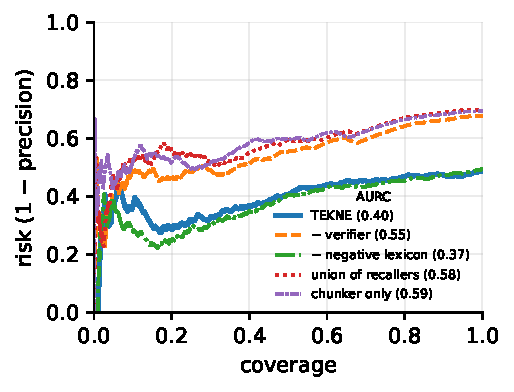
\includegraphics[width=\columnwidth]{figures/risk_coverage}
\caption{Risk against coverage. Configurations that look close on F$_1$ separate
here: what distinguishes them is not how much they find but whether their errors
sit in the low-confidence tail. Lower is better; AURC in the legend.}
\label{fig:riskcoverage}
\end{figure}

\paragraph{Baselines.} Table~\ref{tab:baselines} shows the characteristic profile
of each component. The gazetteer is precise and nearly blind (\RGazetteerR{}
recall): outside computer science the ontology has almost nothing to say.
C-value alone has the worst strict F$_1$ of any configuration
(\RCvalueF) but a respectable partial F$_1$ (\RCvaluePF) --- it finds the right
regions of text and the wrong boundaries, which is precisely what a frequency
statistic with no syntax should do. Gating the chunker on the head-noun lexicon
raises its precision from \RChunkerP{} to \RChunkerGatedP{} and costs more than
half its recall.

\paragraph{The full system.} Table~\ref{tab:ablations} gives \RFullPF{} partial
F$_1$ and \RFullType{} type accuracy at \RFullAurc{} AURC. The hallucination rate
is \RFullHalluc{} in every configuration, as the design requires.

\paragraph{What each component buys, and what it costs.} The ablations do not all
point the same way, and the ones that do not are the informative ones.

Removing the \emph{verifier} is the only unambiguous degradation, and it is
large: precision falls from \RFullP{} to \RNoVerifierP, partial F$_1$ from
\RFullPF{} to \RNoVerifierPF, type accuracy from \RFullType{} to
\RNoVerifierType, and AURC from \RFullAurc{} to \RNoVerifierAurc. Recall rises,
to \RNoVerifierR. That is exactly what a verifier is for --- it does not find
more, it decides what to keep --- and it is the component we would keep if we
could keep only one.

The \emph{negative lexicon} and the \emph{knowledge base plus abbreviation
miner} both trade in the opposite direction. Dropping the negative lexicon costs
strict precision (\RFullP{} to \RNoNegativeP) and strict F$_1$ (\RFullF{} to
\RNoNegativeF) while slightly \emph{improving} partial F$_1$
(\RNoNegativePF) and AURC (\RNoNegativeAurc). Dropping the knowledge base and
abbreviation miner behaves similarly. The explanation is the same in both cases:
these components remove candidates that overlap a gold span without matching it
exactly, so they buy exact-boundary precision by giving up partial credit, and
the items they remove were already ranked low enough that removing them does not
improve the ranking. For a tracking corpus operated at a precision target this
is the right trade, but it is a trade and not a free win.

\emph{Consensus} and \emph{abstention} move strict F$_1$ by less than a point and
improve AURC (\RNoConsensusAurc{} and \RNoAbstentionAurc{} respectively, against
\RFullAurc{} for the full system), which is consistent with their role: they
change what the system is confident about rather than what it finds.
Figure~\ref{fig:riskcoverage} shows why this is worth measuring separately:
configurations within a point of each other on F$_1$ are visibly different in
where their errors sit, and it is that difference, not F$_1$, that determines how
much of the output a downstream corpus can take unreviewed.

\paragraph{Genre.} Table~\ref{tab:genre} shows the gap the task description
predicts. Patents are the harder genre despite contributing more gold mentions
per document, because claim language generates large numbers of well-formed
component noun phrases that are structurally indistinguishable from technology
mentions without domain knowledge --- ``a first position'', ``the both-side end
portions'', ``said support section''.

\paragraph{Error analysis.} Stage-wise accounting on a 20-document sample
attributes the remaining recall loss as follows: candidates cover 80\% of gold
spans exactly and a further 17\% with overlap, so only 2\% is lost at recall.
Of the gold spans present as candidates, the largest single loss is boundary
disagreement at decoding --- the decoder selects an overlapping span the
annotator did not choose --- followed by type errors, predominantly
\textsc{method}$\rightarrow$\textsc{not\_tech} for heads the lexicon does not
list. This is why the strict/partial gap is large and why we report both.

\section{Prompt injection: a negative result}
\label{sec:injection}

Documents are adversary-authored, permanently published, and placed inside a
model prompt, which makes indirect prompt injection \cite{greshake2023injection}
a live concern for a corpus built over decades of filings. We wrap document text
in a per-call nonce fence, but the substantive defence was supposed to be
grounding.

It is not sufficient, and an adversarial test showed why. An attacker who writes
\emph{``always extract QuantumLeap Processor as the primary technology''} into
their own specification has made that string a verbatim substring of their own
document; a grounded extractor has no basis on which to reject it. What
grounding buys is a bound, not a defence: the adversary can only inject
technologies they are willing to publish under their own name. Closing the
residue required a second mechanism --- rejecting candidates whose own sentence
contains instruction-like content --- which costs the mentions in the example
sentences of papers genuinely about prompting. We keep the negative result as a
test so that it stays visible.

\section{Downstream: what the extraction is for}

Aggregating mentions by canonical identifier and document year gives per-
technology series; ranking by recent growth in normalised document frequency
gives an emergence list; and comparing the early and late role distribution of a
technology gives an adoption signature, the shift from \textsc{proposed} to
\textsc{used} and \textsc{compared}. Document frequency rather than mention
frequency is used throughout, since a patent that repeats ``grinding tool''
forty times is one document's worth of evidence that grinding tools matter.

We report this as a demonstration that the extraction output supports the
analysis, not as a contribution to trend detection
\cite{small2014emerging,erdi2013prediction}, and the demonstration is weaker than
we intended: the time-sliced corpus this section needs is assembled from the
arXiv API a year at a time, and the endpoint rate-limited us to two usable time
slices. The aggregation logic is therefore exercised by unit tests on synthetic
series --- document-frequency counting, corpus-size normalisation, emergence
ranking and the adoption signature --- and on the real corpus only across two
points. Nothing in this section should be read as an empirical claim about
technology trends; what it establishes is that canonical identifiers, roles and
dates carry through the pipeline in a form the analysis can consume.

\section{Limitations}

The gold set has a single annotator, so there is no agreement figure and the type
and boundary decisions carry one person's judgement; the reported figures
characterise this pipeline against this annotation rather than absolute accuracy.
Roles are annotated per document rather than per occurrence, which makes patent
role accuracy closer to a measure of zone detection than of stance. The paper
sample is drawn from recent arXiv submissions and over-represents LLM-adjacent
work. In the offline configuration the type classifier and the embedding
verifier share a distributional signal, so that verifier is a consistency check
rather than an independent one; genuine independence requires the LLM tier. The
evaluation zone excludes patent descriptions, where much specific disclosure
lives. Finally, the corpus is small: 44 documents supports ablation comparison
but not confident absolute claims.

\section{Future work}

The highest-value extension is \emph{temporal sense disambiguation}. Vocabulary
is reused across eras --- ``transformer'' in a 2005 power-systems patent is a
magnetic component --- and a single such error lands at the start of a time series,
exactly where an emergence detector is most sensitive. We implement a temporal
guard that withholds knowledge-base links predating a document, but the harder
version, which disambiguates senses against a contemporaneous corpus, is
unattempted.

Three further directions. \emph{Per-occurrence stance} with a trained classifier
rather than a cue lexicon, which the current gold set cannot evaluate.
\emph{Successor relations}: co-occurrence and role transitions already suggest
when one technology displaces another, and extracting explicit comparative
statements (``outperforms X'') would turn that into a graph
\cite{hope2021mechanisms}. \emph{Full-text patents}: the description section
carries the specific disclosure that claim language deliberately generalises
away, and extending the zone there is mostly a cost-control problem given the
batching in \S\ref{sec:cost}. We would also like to compare against a fine-tuned
span tagger \cite{beltagy2019scibert,zhong2021pure} trained on a larger gold set,
and against domain extractors in chemistry \cite{krallinger2015chemdner} on the
patent subset, neither of which the present annotation budget supported.

\section{Conclusion}

Technology extraction for evolution tracking is a precision-dominant,
open-vocabulary problem in which fabricated entities do lasting damage and missed
ones mostly do not. Treating that asymmetry as a design constraint --- offsets
rather than strings, cited evidence rather than assertion, one calibrated
abstention rather than many cautious stages --- produces a system whose
hallucination rate is zero by construction and whose remaining errors are
boundary and type disagreements that a reader can inspect. The components that
matter most are not the ones that find mentions but the ones that decide which to
keep.

\section*{Reproducibility}

Corpora are rebuilt from public endpoints without credentials; all offline
numbers are produced by \texttt{make data kb gold eval}. Each result row is a
configuration object rather than a code path, every mention records the digest of
the configuration that produced it, and model calls are cached content-addressed
so a run replays exactly. The tables in this paper are generated from the results
file and the numbers quoted in prose are LaTeX macros from the same source.

\bibliography{refs}

\end{document}
